%
\section{Grouping and labeling}
%
% Remember to mention that video quality isn't used after phase 1 due to the side effects cased by labeling the video (namely that bad quality segments don't receive any labels). in a real world application this quality measure could be used to reduce the amount of data to analyze

%
\subsection{Literature Study}
%
% describe Haar cascade classifiers (performance and an outline of how they work)
Detecting suitable regions in the video-clips is not enough. The content in the regions also has to be interesting. Hanjalic, A. \cite{citeulike:405480} describes a way to identify such regions by measuring the level of excitement in a sports video-clip based on a manually selected set of features. These features can be both visuals (like the movement in an image or the change of camera positions) or audial (namely the energy contained in the audio track).% WHETHER SUCH AN APPROACH IS SUITABLE TO US IS YET TO BE DETERMINED BASED ON THE CONTENT IN OUR FUTURE DATA SET.
%
\subsection{Method}
%
% how we implemented the Haar cascade classifier

%
\subsection{Detecting interesting regions in video-clips}
%

%
\subsection{Metadata}
%
Before we attempt to label the content in the videos we first extract all the metadata we can. MOOOORE....
%
\subsubsection{Facial Detection}
%
With the introduction of Haar cascade classifiers by Viola and Jones \cite{viola01}, later improved upon by Lienhart and Maydt \cite{lienhart01}, we have a very efficient tool for facial detection. OpenCV provides an implementation of an already trained classifier, manifested as a range of xml-files describing the Haar like features of a human face, both front and profile, aswell as upper body, lower body, and full body (CONFIRM!!!!!).\\
Describe how Haar Cascade Detection works?\\
The Haar Cascade Classifier uses a data-structure called an integral image, an algorithm based on AdaBoost that selects critical visual features, and a method that combines complex classifiers to compute on the most promising object-like regions.\\
An integral image is a matrix where any point $(x,y$ is the sum of all pixels above and to the left of $(x,y)$. Not only is the computation of this matrix efficient as a function of its nature (it can reuse already computed sums when building the matrix), the sum at any given point can be computed in constant time as it can be done by 4 lookups in the matrix followed by 4 additions and substractions. A FIGURE WOULD ILLUSTRATE THIS QUITE WELL.\\
AdaBoost (Adaptive Boosting) is a meta-algorithm for boosting machine learning algorithms where subsequent classifiers built are tweaked in favor of those instances misclassified by previous classifiers (partly FROM WIKI). The derivative algorithm is a modification of AdaBoost that constrains each returned (weak) classifier to be dependent only on a single feature, which in turn is deemed a critical feature.\\
A method of using less complex processing to detect promising regions, and then apply the more complex processing on these regions.
%
\subsubsection{Brightness}
%
The brightness of a video is expressed as an array of means of the color intensity through all frames in the video. Since the videos have already been converted to grayscale at this point in the pipe-line this is a trivial task, due to there only being a gray channel in the pixels.
%
\subsubsection{Optical Flow}
%
% TODO: Move this section below Shift Vector Magnitude
%
% TODO: Describe Optical Flow in general
%
Our experiments with Optical Flow are based on a wish to extract information about was is happening in the video. Whereas the Shift Vector Magnitude tells us something about how the camera itself moves, Optical Flow attempts to explain how the content within each frame moves. There has been a substancial amount of research put into this field. [REFS] describes ways to identify certain types of actions occuring within videos, such as violent behaviour, [REF] looks at general crowd movement in public places, and [REF] describes how Optical Flow can be used to identify pedestrians, even at great distance where such methods as Facial- and People- Detection come up short, in conection with the navigation of autonomous vehicles.\\
%
One huge difference between our work and that of all the previous research we have been able to find is that we do not have the luxary of a stationary camera, or, in the case of the autonomous driving researh in [REF], at least a fixed camera. Most of our footage is recorded by handheld cameras often under very poor conditions. Extracting the optical flow of our videos is therefore not only a matter of analysing how reference points move around in the frame. First we need to \textit{stabilise} the frame itself.\\
%
\paragraph{Frame stabilisation}
%
There are several obvious ways to do this, but each has their own limitations. The first that comes to mind is to simply use the Shift Vector Magnitudes that we have already computed. This intuitively makes a lot of sense since they are suppose to tell us exactly how the camera moves at each point of the video. Thus, it should simply be a matter of subtracting this general movement from whatever individial movement is detected within the frame and the remaining movement would be the optical flow of the content. However, it turns out that although the Shift Vector approach is very suitable for describing the general type of cameara movement (shaking, panning), especially when the data is smoothed across several frames, it has a relatively high margin of error for individual frames. This is especially the case if the camera moves very fast or if there actually \textit{is} a lot of movement within the frame. Other approaches [REF] involve calculating the optical flow and then subsequently subtracting the mean of all the individual vectors it yields, from the each of the vectors. Yet another way [REF] is to detect the most dominant vector direction and use that as a stabiliser. However, all our experimentation showed that these methods suffer from one serious limitaion. If moving objects in the frame a very close to the camera, they tend to become more influencial than the stationary background and they end up swapping roles. The very movement we want to extract is removed and everything we would like to get rid of remains. The border-case for this condition is especially problematic. This occurs when an object is at the exact distance from the the camera where it \textit{periodically} becomes the dominant set of movement. In these cases the stabilising vector will jump from one extreme to the other and thus be completely useless.\\
Some of these problems could probably be alleviated through further analysis or averaging across time, however, through our experimentation we came up with an approach that seems quite promising.\\\\
%
We noticed that a preliminary detection of Good Features to Track was very beneficial. The method, described by [REF] is based around detecting pixels (or \textit{corners}) in an image, that has high eigenvalues. These points has a tendency to be present in stationary objects in the frame far more often than in moving objects, and thus form a very decent base for our stabilising vector. We chose to simpy calculate the mean of these vectors and use that, although it also would be possible to detect the most common direction as described above and in [REF].
%
% REMEMBER: Describe RISKS (zooming)
\subsubsection{Blue channel}\label{sec:blue_channel}
%
Each frame in a video consists of a matrix of pixels in 3 channels, red, green, and blue. For the purpose of police detection, described in detail in section \ref{sec:police_detection}, and day/night detection, described in detail in section \ref{blah}, we extracted the blue channel in each frame and computed the mean pixel intensity. 
%
\subsubsection{Contrast}
%
Some of the metadata is already extracted in earlier phases. The contrast is an example of this. The contrast in a frame is defined as being the standard deviation of the color-intesity values in the image-matrix. A small deviation would indicate little contrast/diversity in color-intensity, and a large deviation would indicate a high contrast/much diversity in color-intensity. Again, the contrast metadata for each video is expressed as an array of these standard deviations in each frame.
%
\subsubsection{Shift Vector Magnitude}
%
Like the contrast, the shift vector magnitudes for each video is already computed as a part of the initial image quality assessment. We attempt to estimate the camera movement by \textit{shifting} each frame until its content more or less alligns with the content of the previous frame. This shift is expressed as a vector, whos magnitude tells us how much the camera is moving/shaking at each frame point in the video.
%
\subsection{Labels}
%

%
\subsubsection{Police Detection}\label{sec:police_detection}
%
% blue channel mean, local minima/maxima. oscillation
By investigating the blue channel mean, see section \ref{sec:blue_channel}, in detail we are able to some degree detect if the police is present in part of a video, under the circumstance that the police blinker lights are active. The theory was simple: we would expect the blue channel mean to oscilate over time. If we plot the mean values as a function of time (frames) we can easily distinguish oscilating areas visually, and then check if this osciallation corresponds to police being present in the video at that point in time. Somewhat to our surprise this was amazingly accurate. We did get a rather large number of false negatives, but almost no false positives.\\
We did not find any ready-at-hand code for detecting oscillations so we rolled something ourselves. What we ended up with was a simple approach based on the realization that the points in an oscillating graph could be connected by triangular shapes (bottom facing up) see Figure \ref{fig:triangles}, and each consequtive triangle is roughly the same shape and size. The problem was boiled down to matching these triangles.\\
We compute the magnitude of the vectors a,b,c,d,e,f and check if the relative standard deviation of $[a,b,c,d]$ and $[e,f]$ is below a certain treshold (meaning that a,b,c,d and e,f are roughly the same length).
%
\begin{figure}
     \centering
     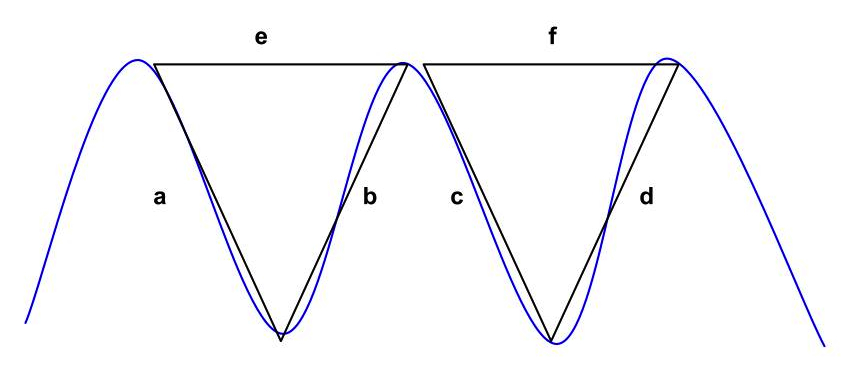
\includegraphics[width=1.05\textwidth]{img/triangles.jpg}
     \caption{}\label{fig:triangles}
\end{figure}
% 
%
\subsubsection{Vertical Oscillation}
%

%
\subsubsection{In crowd}
%
% based on facial detection

%
\subsubsection{Person in Focus}
%
% based on facial detection and object placement in frame (center)

%
\subsubsection{Overview}
%

%
\subsubsection{Day \& Night}
%
% Test/Success-rate